\documentclass{article}
\usepackage[margin=0.6in]{geometry}
\usepackage[utf8]{inputenc}
\usepackage{physics}
\usepackage{graphicx}
\usepackage{siunitx}
\usepackage{amsmath}
\usepackage{amssymb}
\usepackage[numbers,sort&compress]{natbib}
\usepackage{bm}
\usepackage{url}
\usepackage{hyperref}
\usepackage{parskip}
\usepackage{lineno}
\usepackage{float}
\linenumbers

\setlength\parindent{0pt}
\renewcommand{\baselinestretch}{1.5}

\usepackage{authblk}

\title{Optimal time-dependent deployments of climate control technologies}
\author[1,2]{Henri F. Drake\textsuperscript{*}}
\author[1]{Ron Rivest}
\author[1]{Alan Edelman}
\author[1]{John Deutch}
\affil[1]{Massachusetts Institute of Technology, Cambridge, MA, USA}
\affil[2]{Woods Hole Oceanographic Institution, Woods Hole, MA, USA}

\date{}             %% if you don't need date to appear
\setcounter{Maxaffil}{0}
\renewcommand\Affilfont{\itshape\small}

\begin{document}
\maketitle

\section{Model formulation}

\subsection{CO$_{2}$ concentrations: baseline emissions, emissions reductions, and negative emissions}

We assume a baseline emissions scenario which has emissions constant until 2060 and emissions decreasing linearly to zero in 2100:
\begin{equation}
  q(t)=\begin{cases}
        5
        & \text{for $2020 \leq t < 2060$}\\
        5 (1 - \frac{t-t_{0}}{40})
        & \text{for $2060 \leq t < 2100$}\\
        0
        & \text{for  $2100 \leq t$}
       \end{cases} \quad\quad \text{ ppm/year}.
\end{equation}

CO$_{2}$ concentrations start at $\SI{415}{ppm}$ and increase according the emissions scenario $q(t)$.

\subsection{Temperature response}


\subsection{Climate damages}

\subsection{Control costs}

\subsection{Total costs and discounting}

\begin{figure}[htb!]
\noindent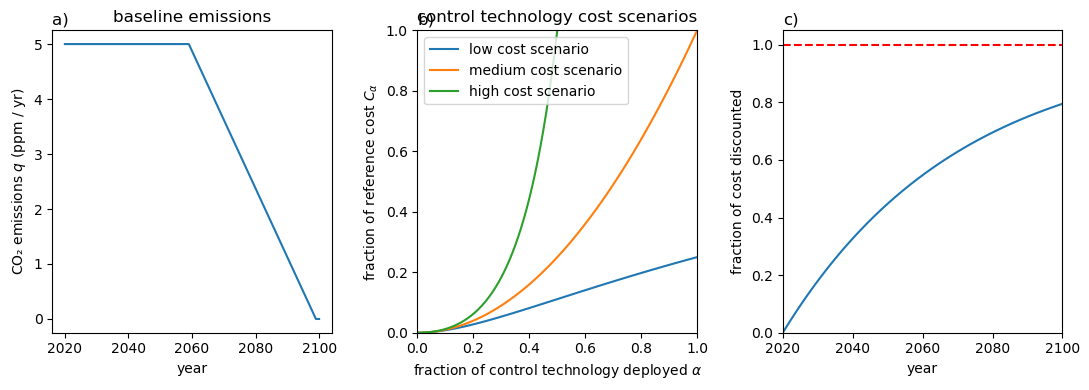
\includegraphics[width=1.0\textwidth]{figures/model_configuration.png}
\centering
\caption{(a) Idealized no-policy baseline emissions scenario. (b) Three different idealized functions for the cost scaling of climate control technologies. (c) The fraction of cost discounted by year under a 2\% utility discount rate.}
\label{fig-configuration}
\end{figure}

%\bibliographystyle{naturemag}
%\bibliography{climate-model-performance.bib,manual_refs.bib}

\end{document}